\documentclass{beamer}


\usepackage[utf8]{inputenc}
\usepackage{amsmath}
\usepackage{amsfonts}
\usepackage{amssymb}
\usepackage{graphicx}
\usepackage{ragged2e}  % `\justifying` text
\usepackage{booktabs}  % Tables
\usepackage{tabularx}
\usepackage{tikz}      % Diagrams
\usetikzlibrary{calc, shapes, backgrounds}
\usepackage{amsmath}
\usepackage{amssymb}
\usepackage{dsfont}
\usepackage{url}       % `\url
\usepackage{listings}  % Code listings
\usepackage[T1]{fontenc}
\usepackage[percent]{overpic}
\usetikzlibrary{trees}
\usepackage[absolute,overlay]{textpos}
\usepackage{tcolorbox}
\usepackage{menukeys}


\newtcolorbox{terminal}{colback=black!70!white,colframe=black!70!white}
\newtcolorbox{focus}{colback=black!10!white,colframe=black!10!white}
\newtcolorbox{terminal2}[1]{colback=white,colframe=black!70!white,fonttitle=\bfseries,title=#1}

\usepackage{theme/beamerthemehbrs}
\usepackage[normalem]{ulem}
\author[MAS]{Hassan Umari}
\title{ROS Services}
\subtitle{Foundation Course}
\institute[HBRS]{Hochschule Bonn-Rhein-Sieg}
\date{\today}
\subject{ROS workshop}

% \thirdpartylogo{path/to/your/image}


\begin{document}
{
\begin{frame}
\titlepage
\end{frame}
}


\section{Recap}
\begin{frame}{Recap}
    \framesubtitle{Summary of yesterday’s session}
    
    \begin{enumerate}
        
        \item We created a ROS \textbf{package} and wrote a ROS \textbf{node} in Python.
        \item We saw how to define a \textbf{publisher} and a \textbf{subscriber} in our node.
        \item We looked into \textbf{launch} files, and ROS \textbf{parameters}.
        \item We saw how \textbf{node names} (or any resource: parameter, topic ..etc) are resolved.
        \item and how to do name \textbf{remapping}.


    \end{enumerate}
\end{frame}

\begin{frame}[fragile]{Recap}
    \framesubtitle{What does this node do?}
    \lstset{language=python,
        basicstyle=\scriptsize,
        keywordstyle=\color{blue}\ttfamily,
        stringstyle=\color{red}\ttfamily,
        commentstyle=\color{green}\ttfamily,
        morecomment=[l][\color{magenta}]{\#},
        showstringspaces=false
    }
    \begin{lstlisting}
    #!/usr/bin/env python
    
    import rospy
    from std_msgs.msg import String
    
    def myfunction(received_msg):
        msg.data = "Hey, I think I heard: " + received_msg.data
        pub.publish(msg)
    
    if __name__ == '__main__':
        rospy.init_node('useless_node')
        
        pub = rospy.Publisher('mouth', String, queue_size=1)
        sub = rospy.Subscriber('ears', String, callback=myfunction)
        
        msg = String()
        rospy.spin()
    \end{lstlisting}
\end{frame}

\begin{frame}{Recap}
    \framesubtitle{Summary of yesterday’s session}
    
    We notice the following:
    \vspace{5mm}
    \begin{enumerate}      
        \item The previous node communicates back and forth with another subscribing node.
        \vspace{5mm}
        \item But is there a better way to make two-way communication between nodes?
    \end{enumerate}
\end{frame}

\begin{frame}{Recap}
    \framesubtitle{Summary of yesterday’s session}
    
    Yes, we can do that with:
    \vspace{5mm}
    \begin{enumerate}      
        \item ROS services.
        \vspace{5mm}
        \item ROS actions.
    \end{enumerate}
\end{frame}

\begin{frame}{Recap}
    \framesubtitle{ROS Concepts}
    
    Concepts related to ROS computation graph:
    
    \begin{enumerate}
        \item \sout{Nodes.}  \checkmark
        \item \sout{Topics.} \checkmark
        \item \sout{Messages.} \checkmark
        \item \sout{Master.} \checkmark
        \item Services.
        \item Actions
        \item \sout{Parameter Server.} \checkmark
        \item Bags.
    \end{enumerate}
\end{frame}

\section{ROS Services}

\begin{frame}{ROS Services}

    {\huge Services:}
    \vspace{0.2cm}
    \begin{itemize}
        \item Communication happens between two nodes, the service \textbf{server} node, and the service \textbf{client} node.
        
        \item A Client node sends a request for a named service and waits for the response, a node serving this service responds, and the communication is over.
        
        \item it is a one-to-one, two-way, one-time communication.
    \end{itemize}  
\end{frame}


\begin{frame}[plain]{}
 \centering
 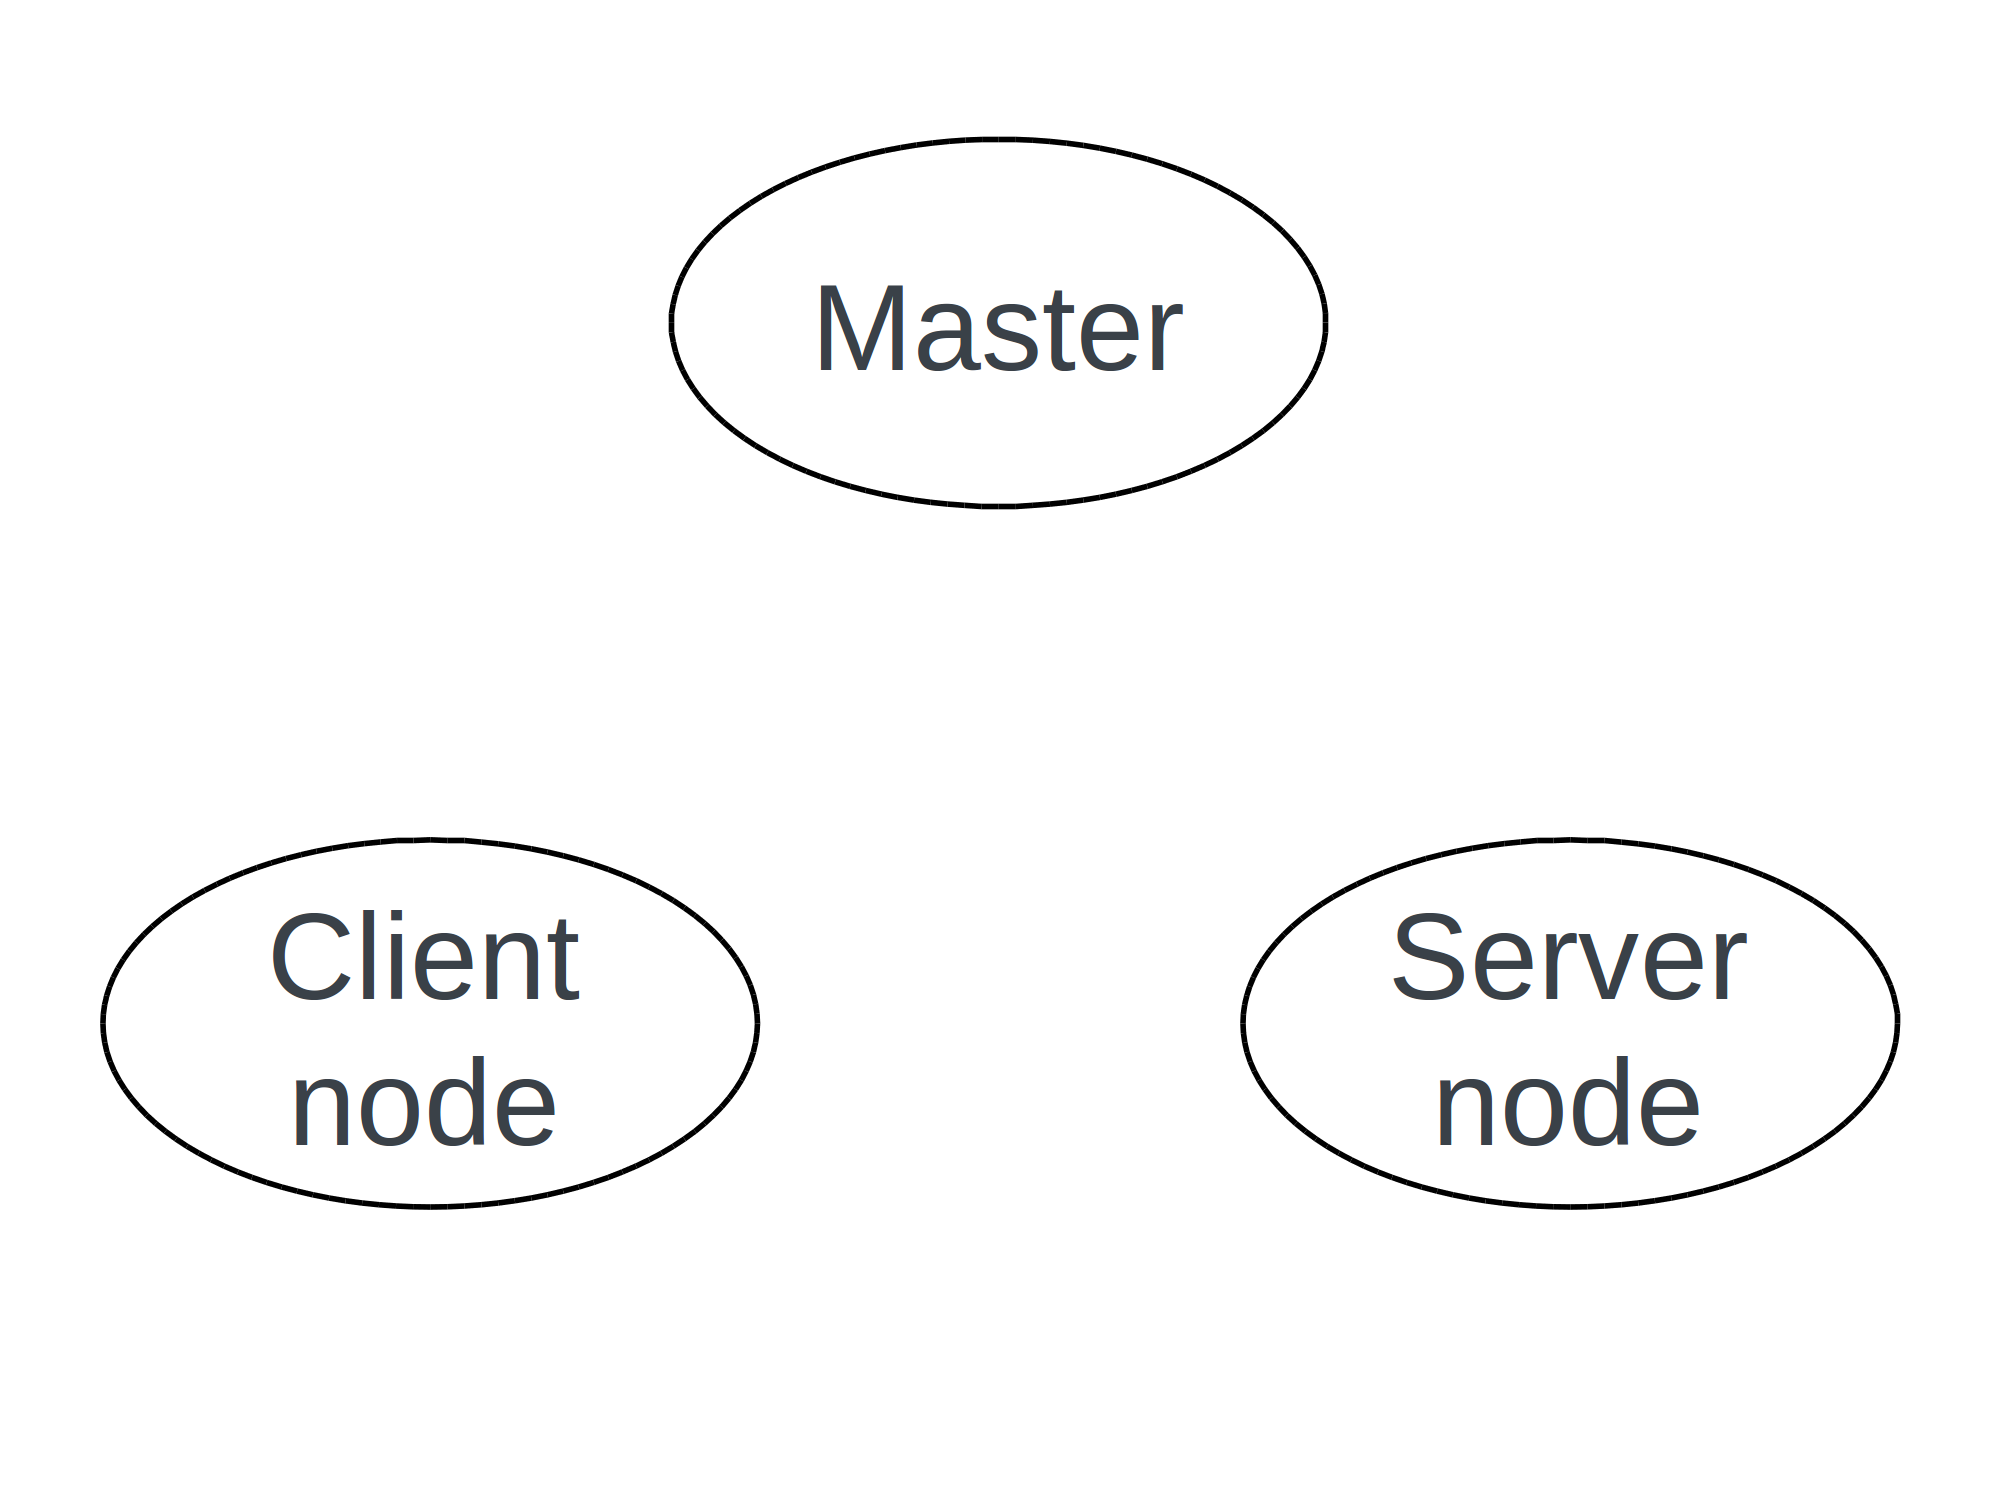
\includegraphics[width =1.0\linewidth]{figures/service1.png}                                                              
\end{frame} 
\begin{frame}[plain]{}
    \centering
    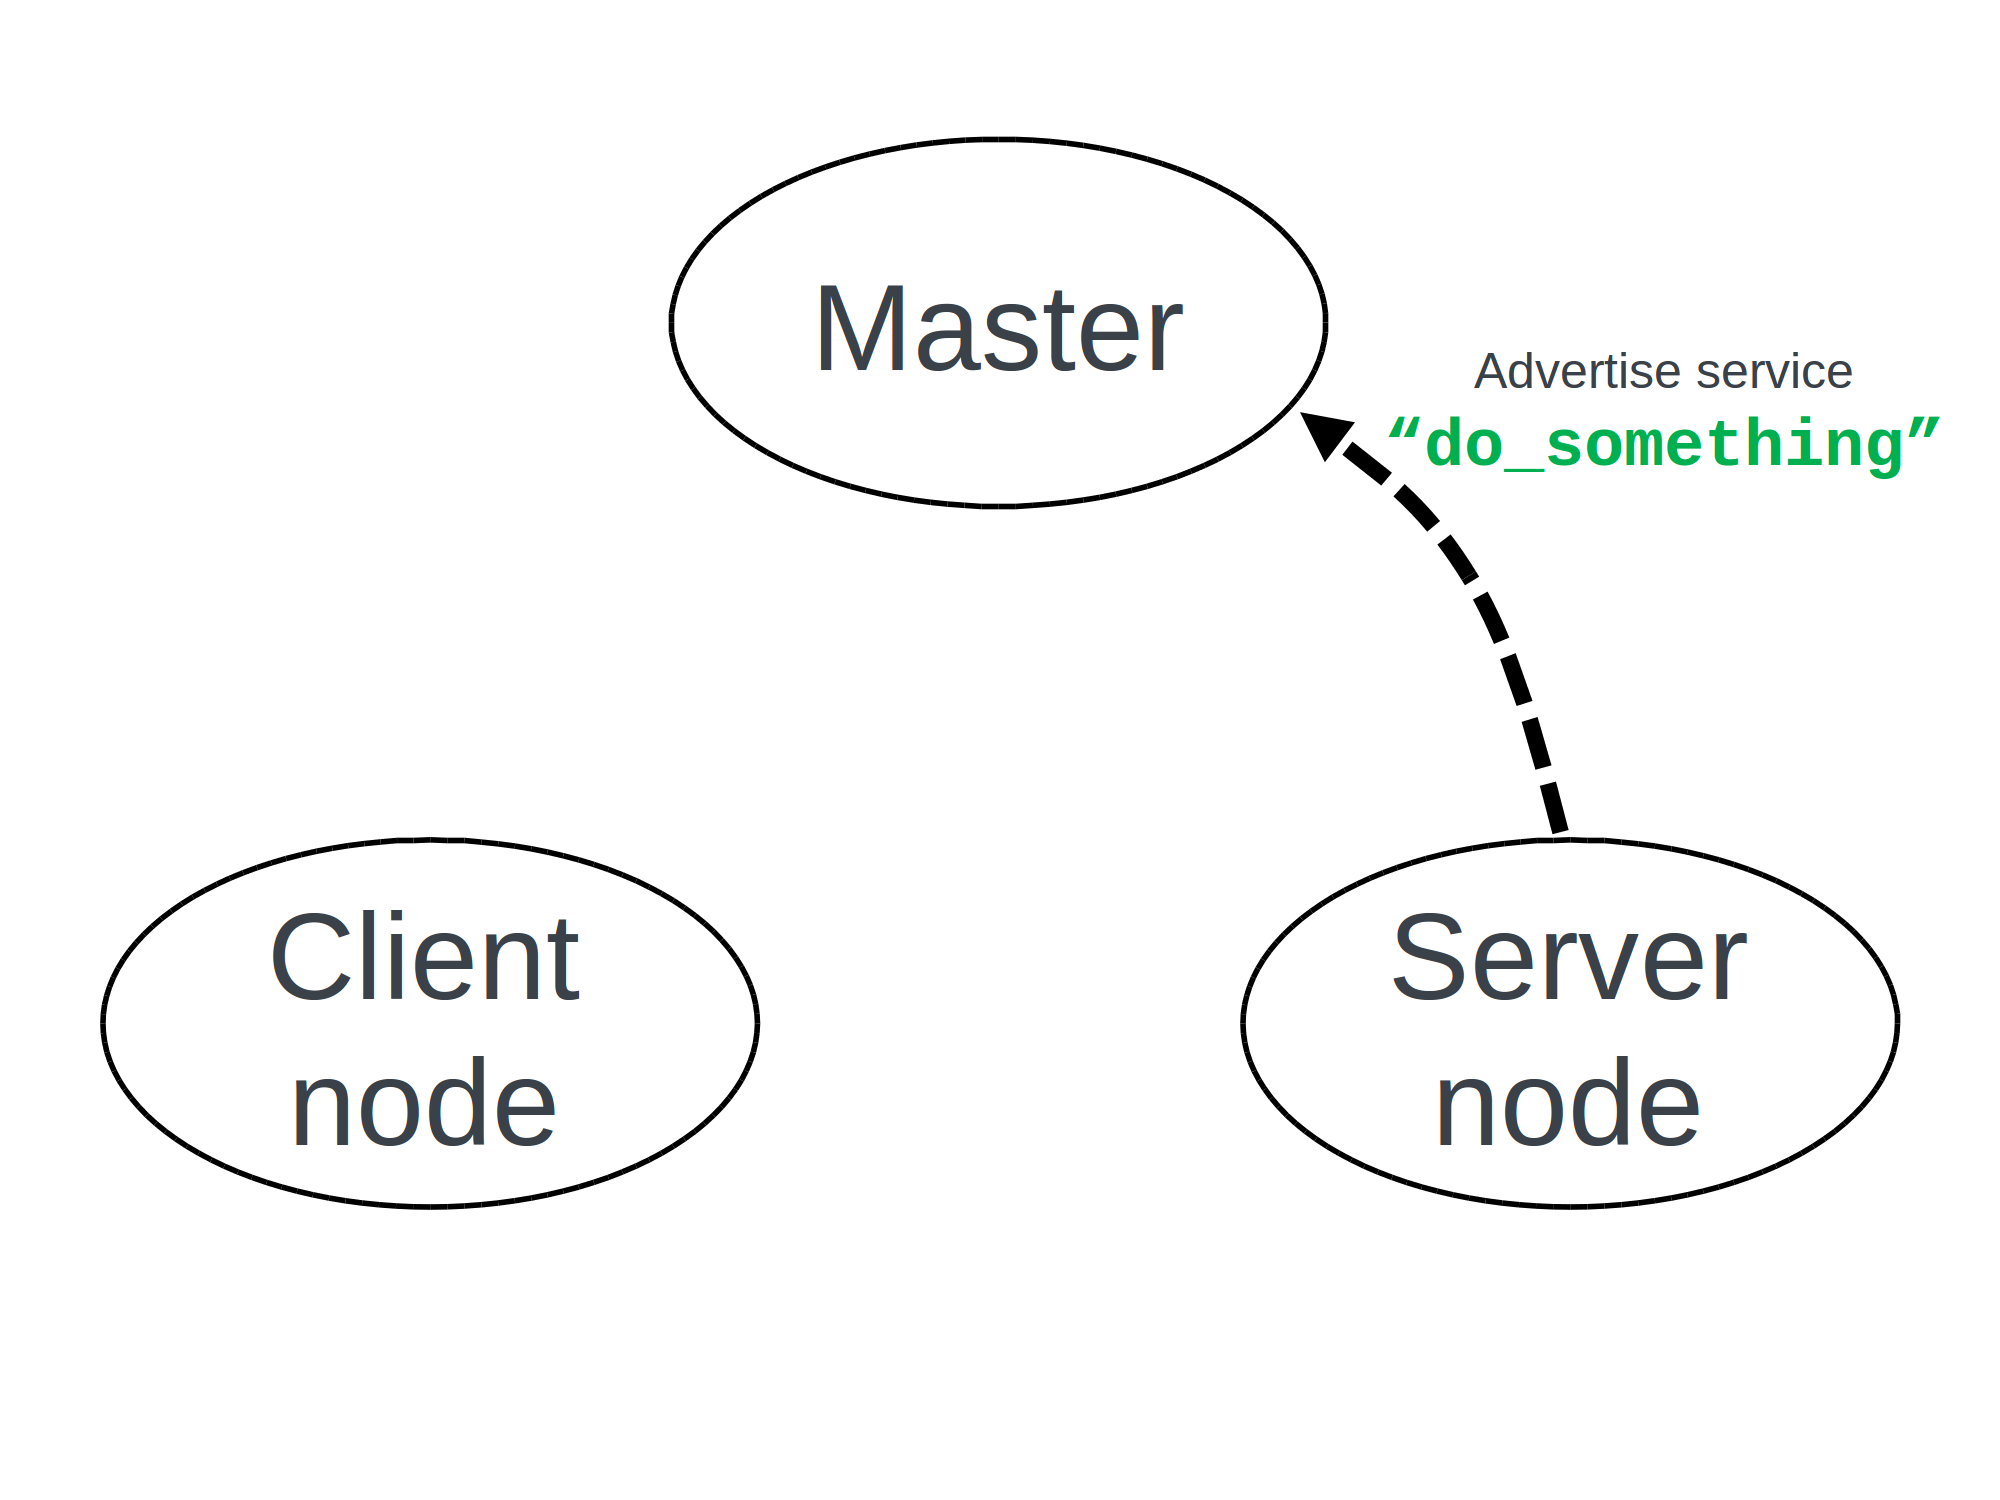
\includegraphics[width =1.0\linewidth]{figures/service2.png}                                                              
\end{frame} 
\begin{frame}[plain]{}
    \centering
    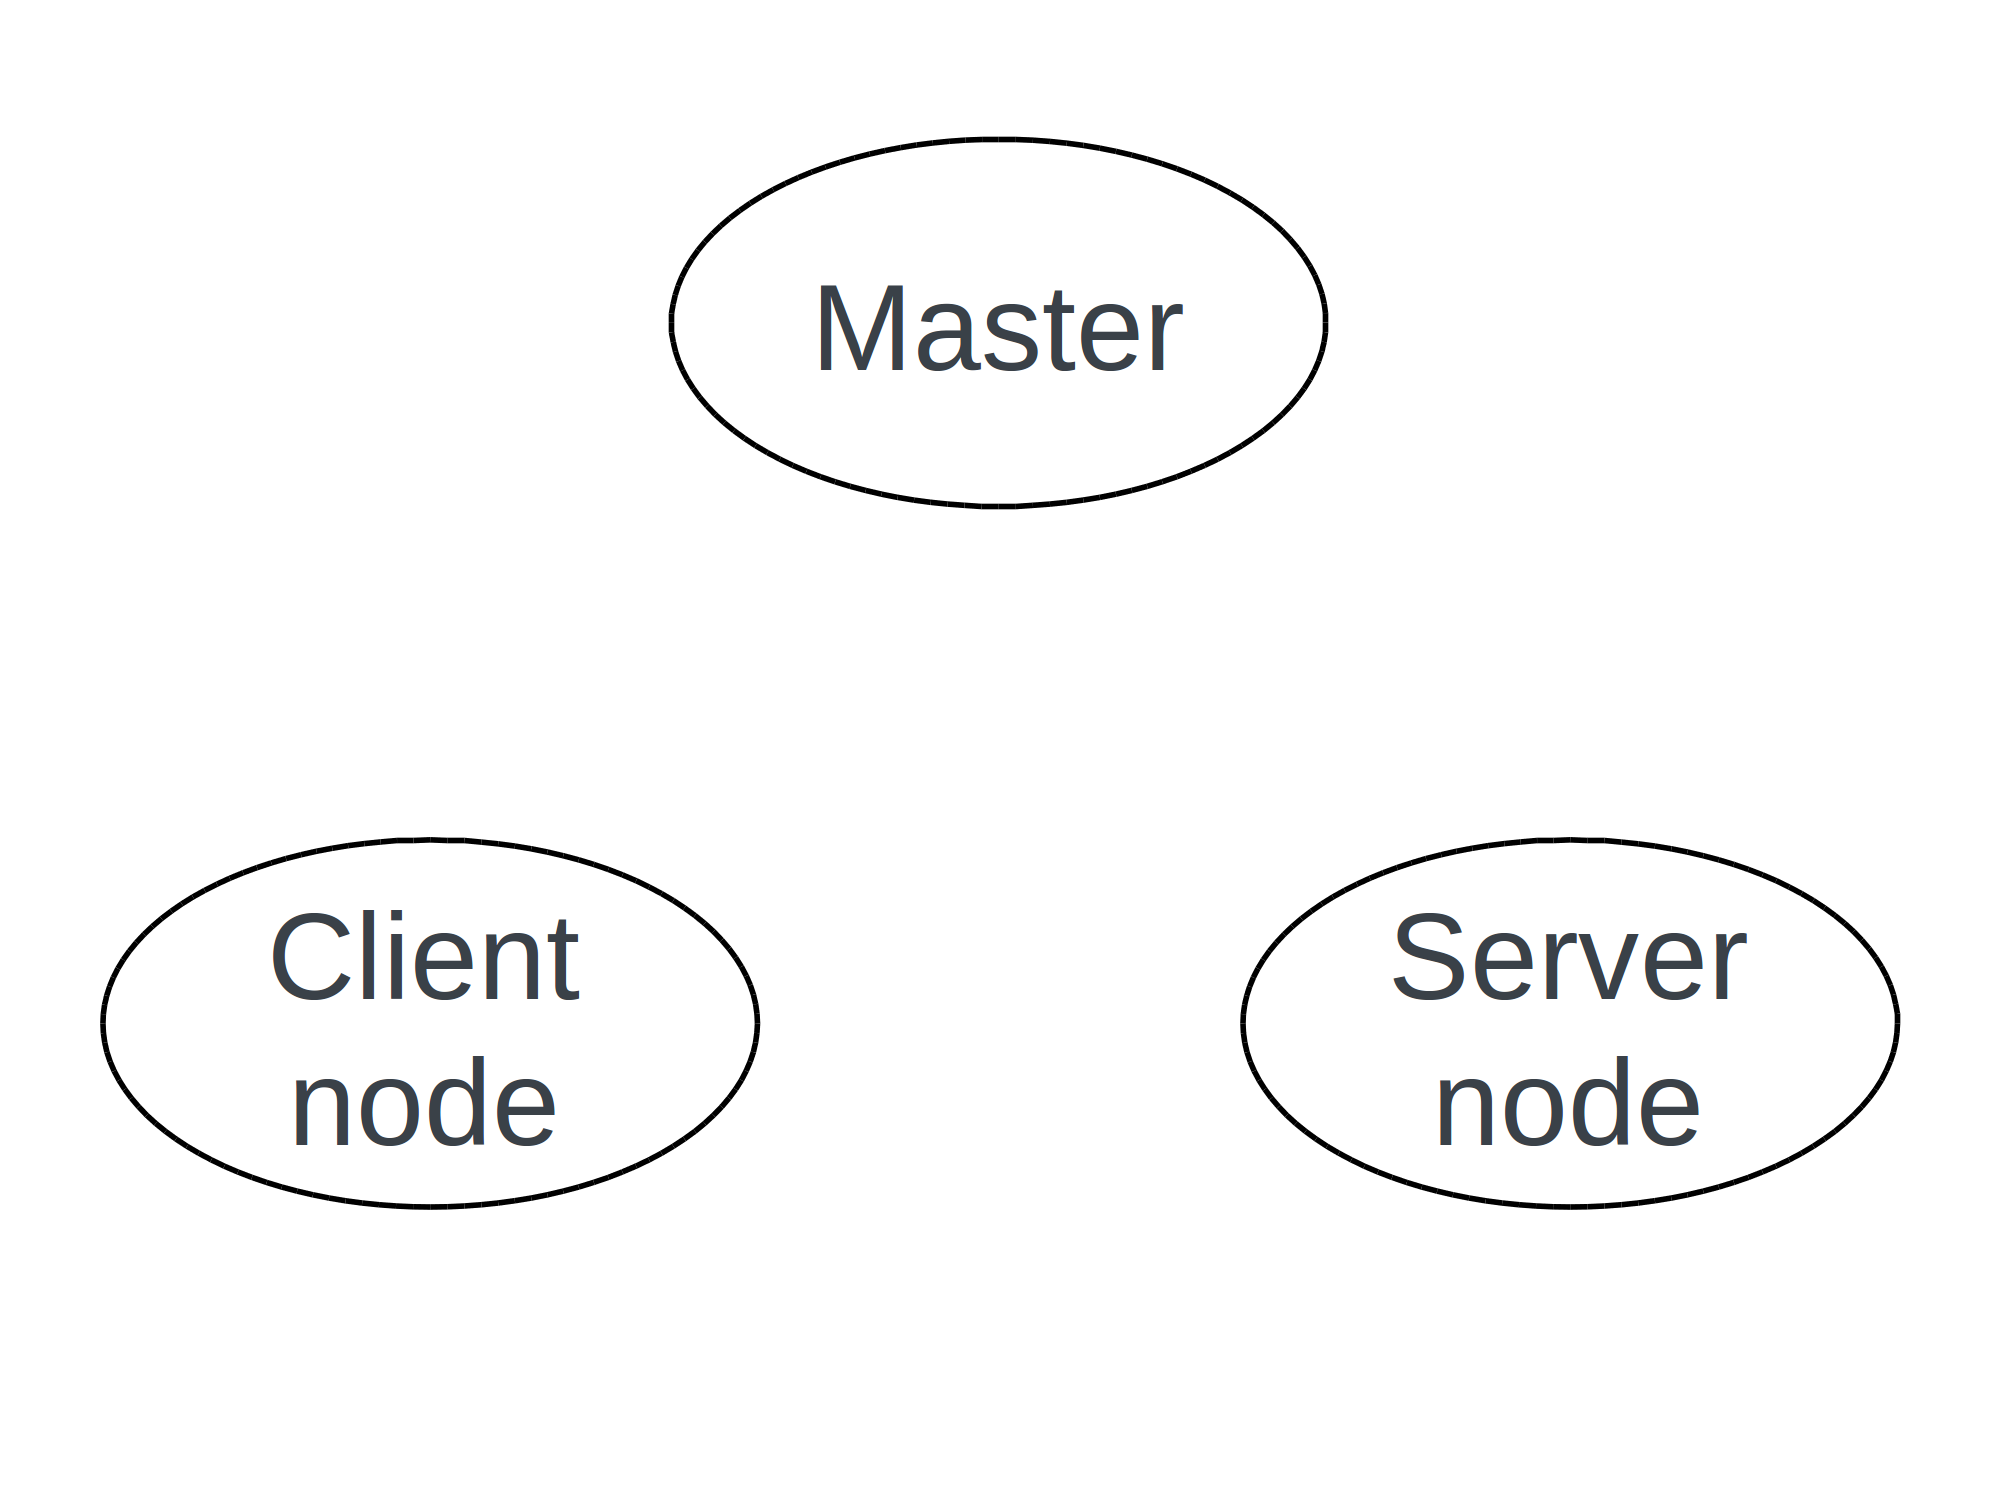
\includegraphics[width =1.0\linewidth]{figures/service1.png}                                                              
\end{frame} 
\begin{frame}[plain]{}
    \centering
    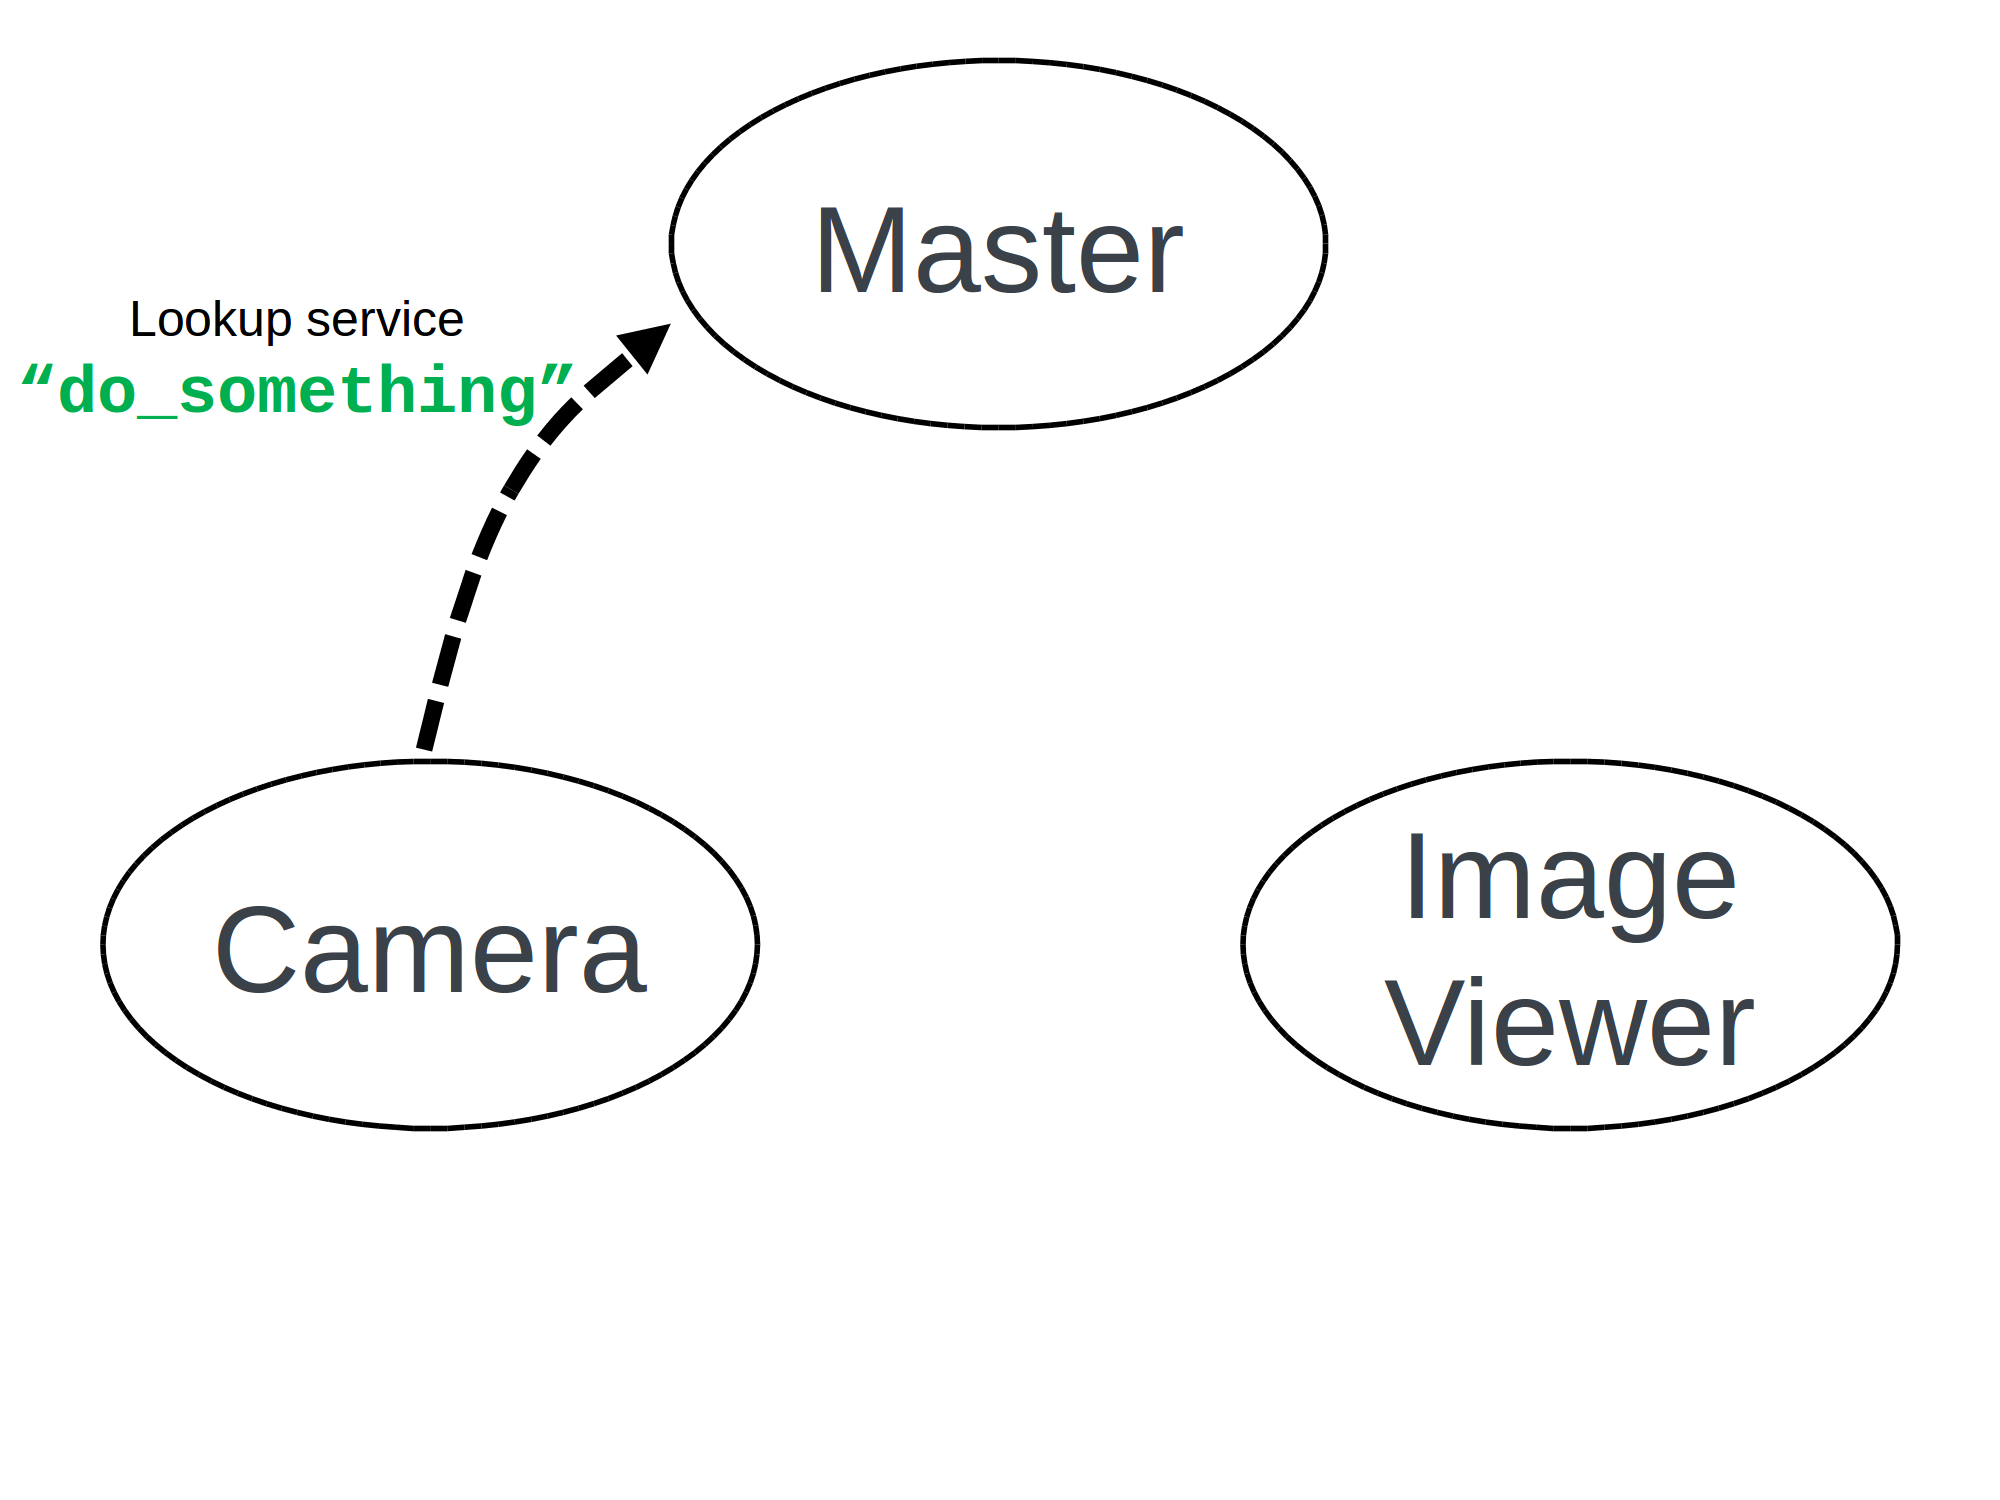
\includegraphics[width =1.0\linewidth]{figures/service3.png}                                                              
\end{frame} 
\begin{frame}[plain]{}
    \centering
    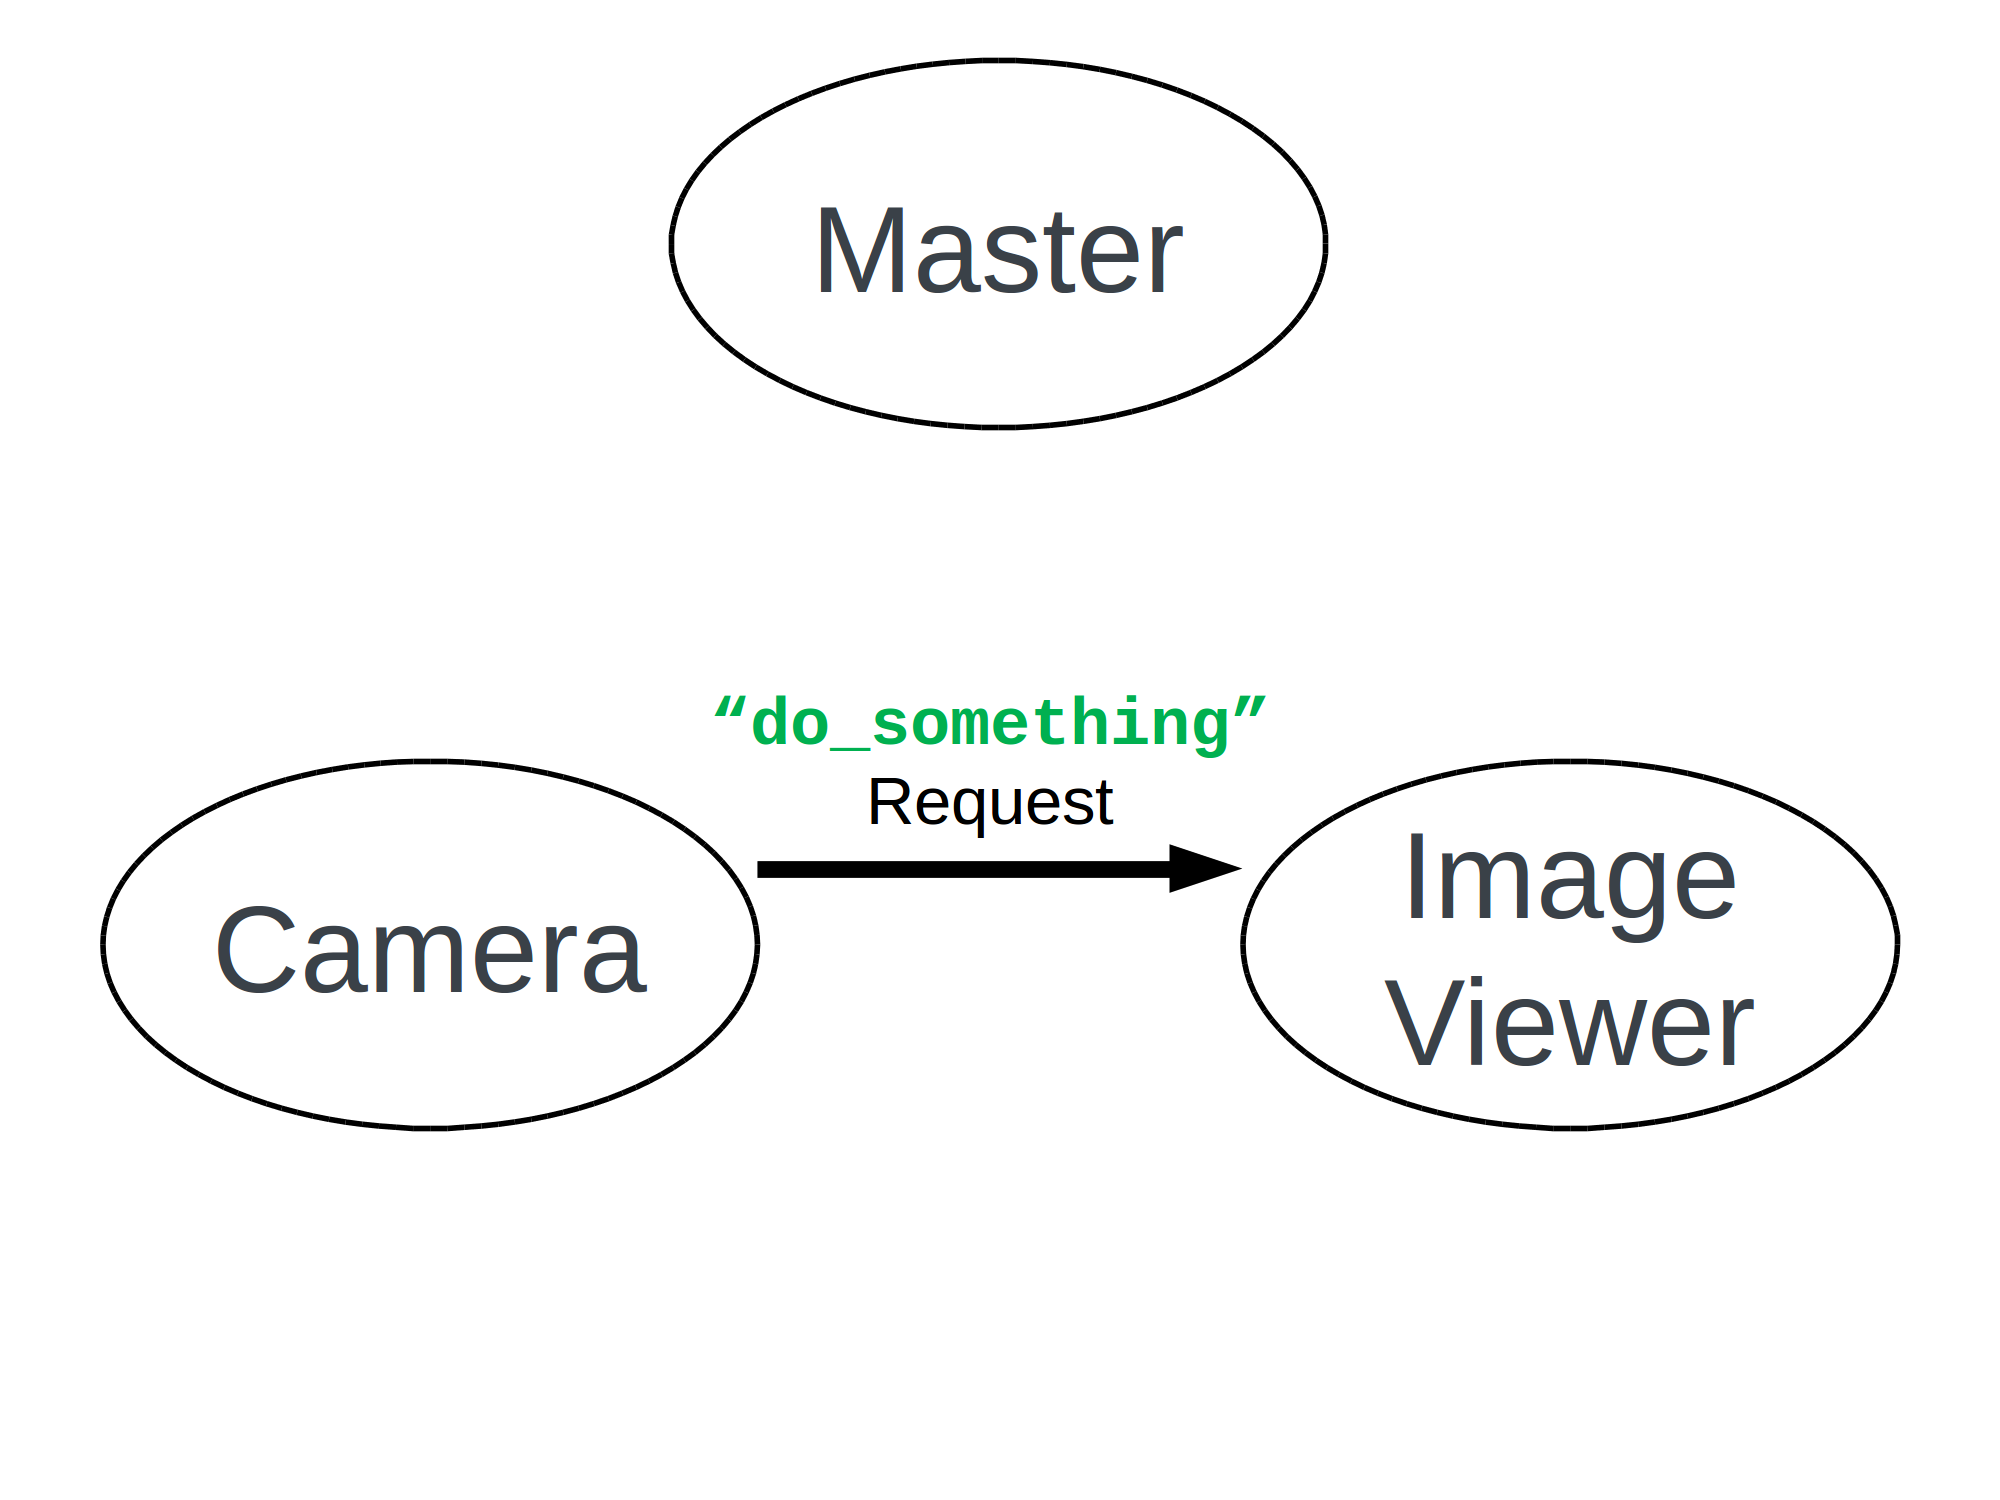
\includegraphics[width =1.0\linewidth]{figures/service4.png}                                                              
  \end{frame} 
\begin{frame}[plain]{}
    \centering
    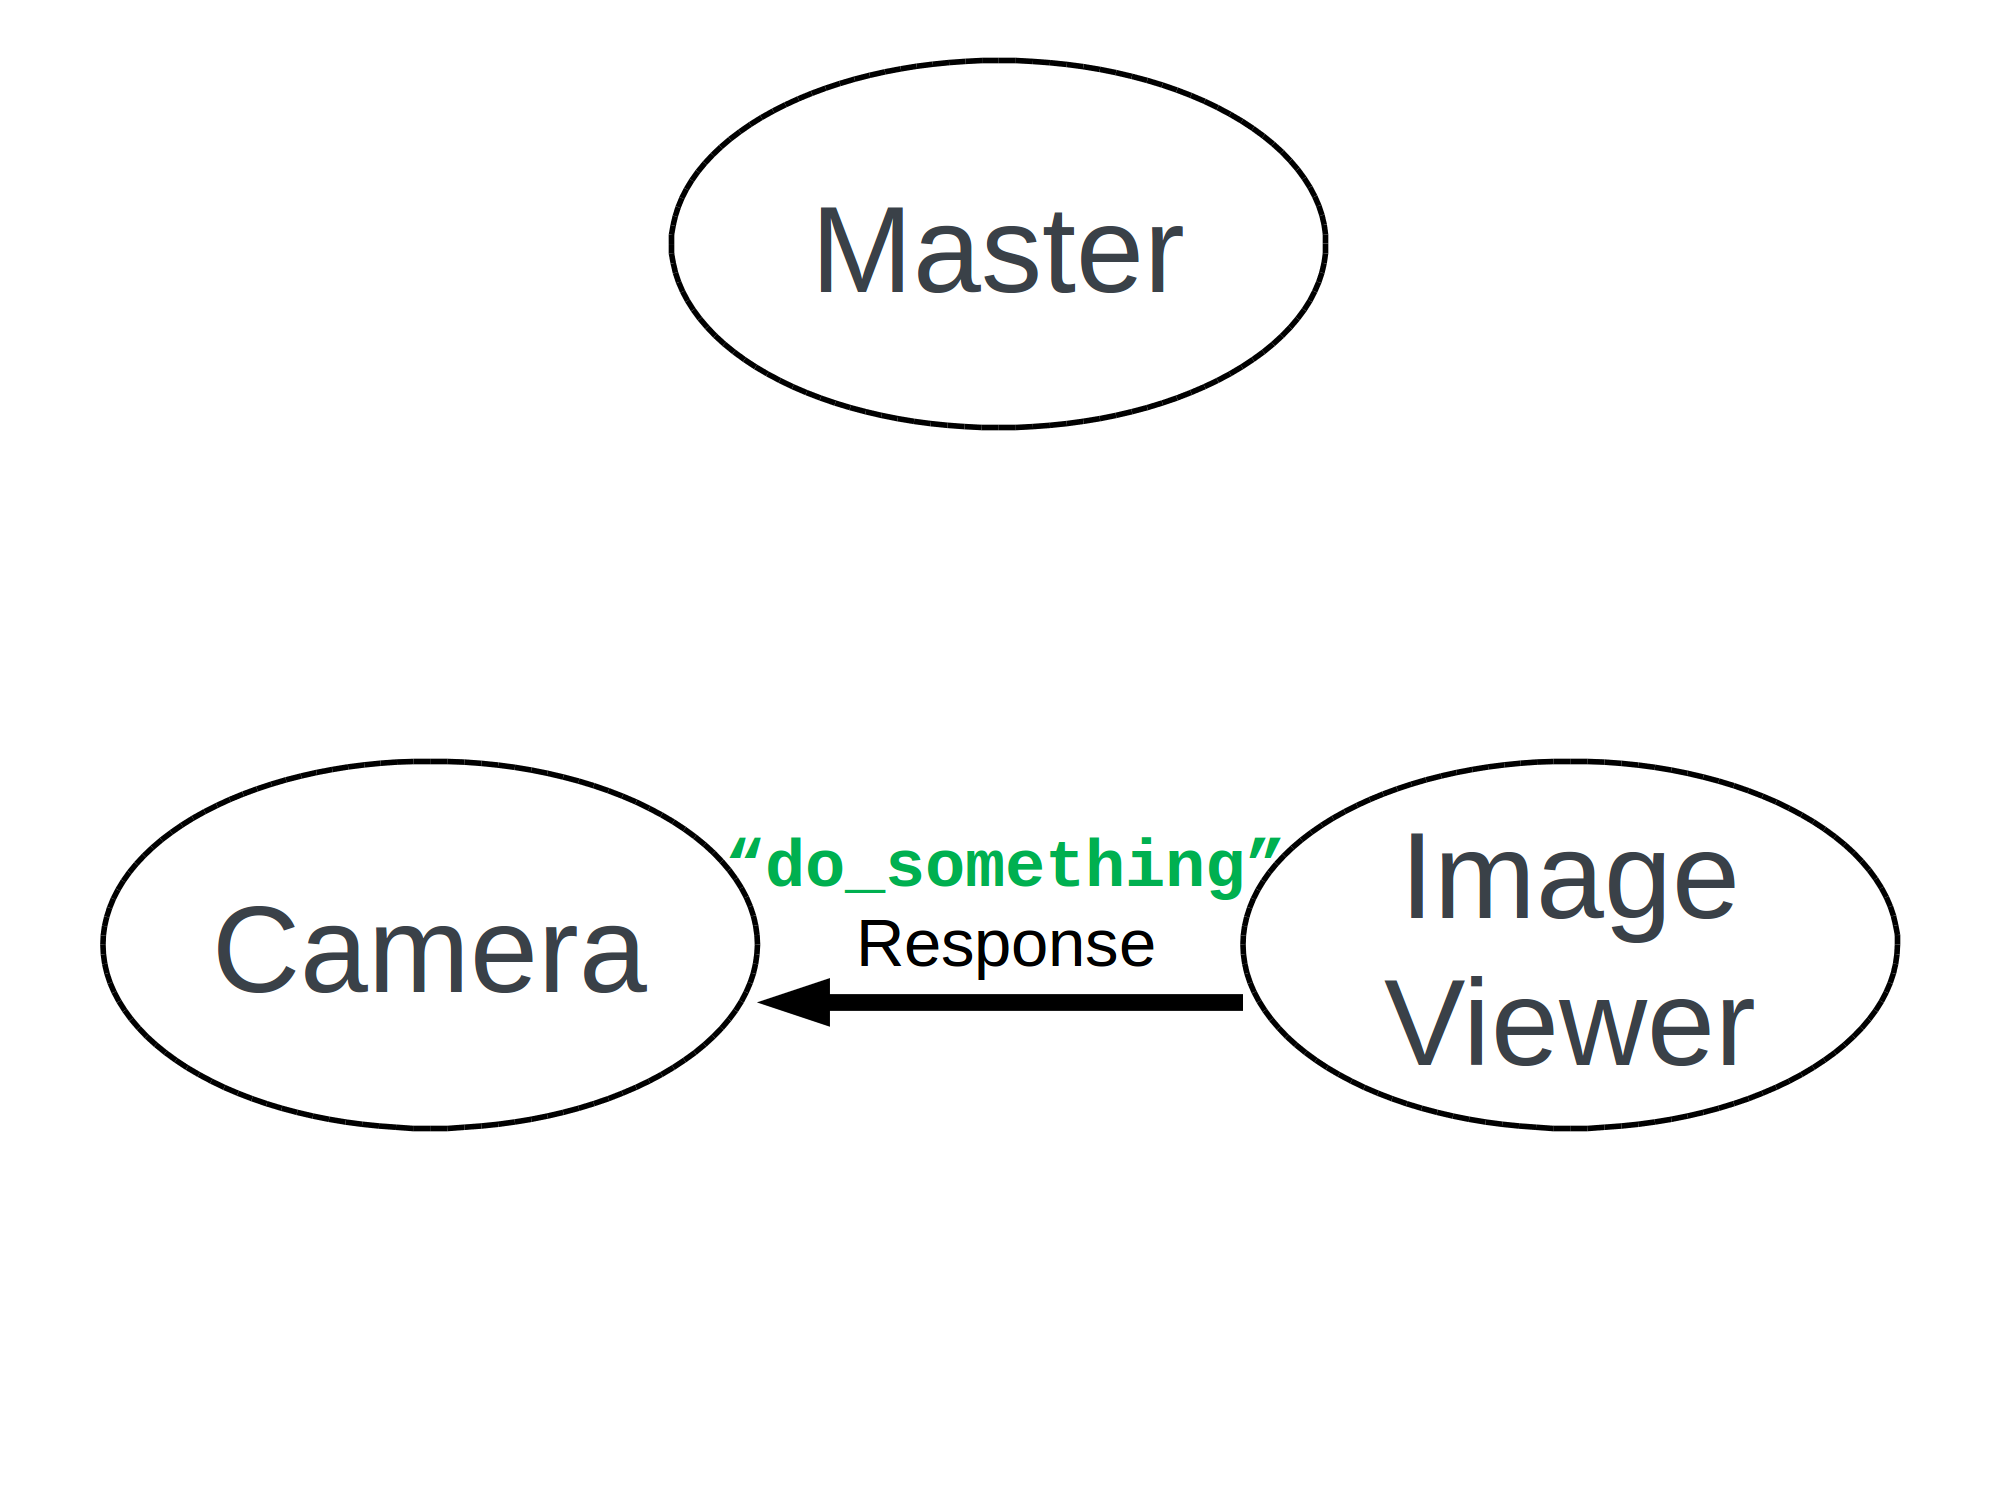
\includegraphics[width =1.0\linewidth]{figures/service5.png}                                                              
  \end{frame}
\begin{frame}[plain]{}
    \centering
    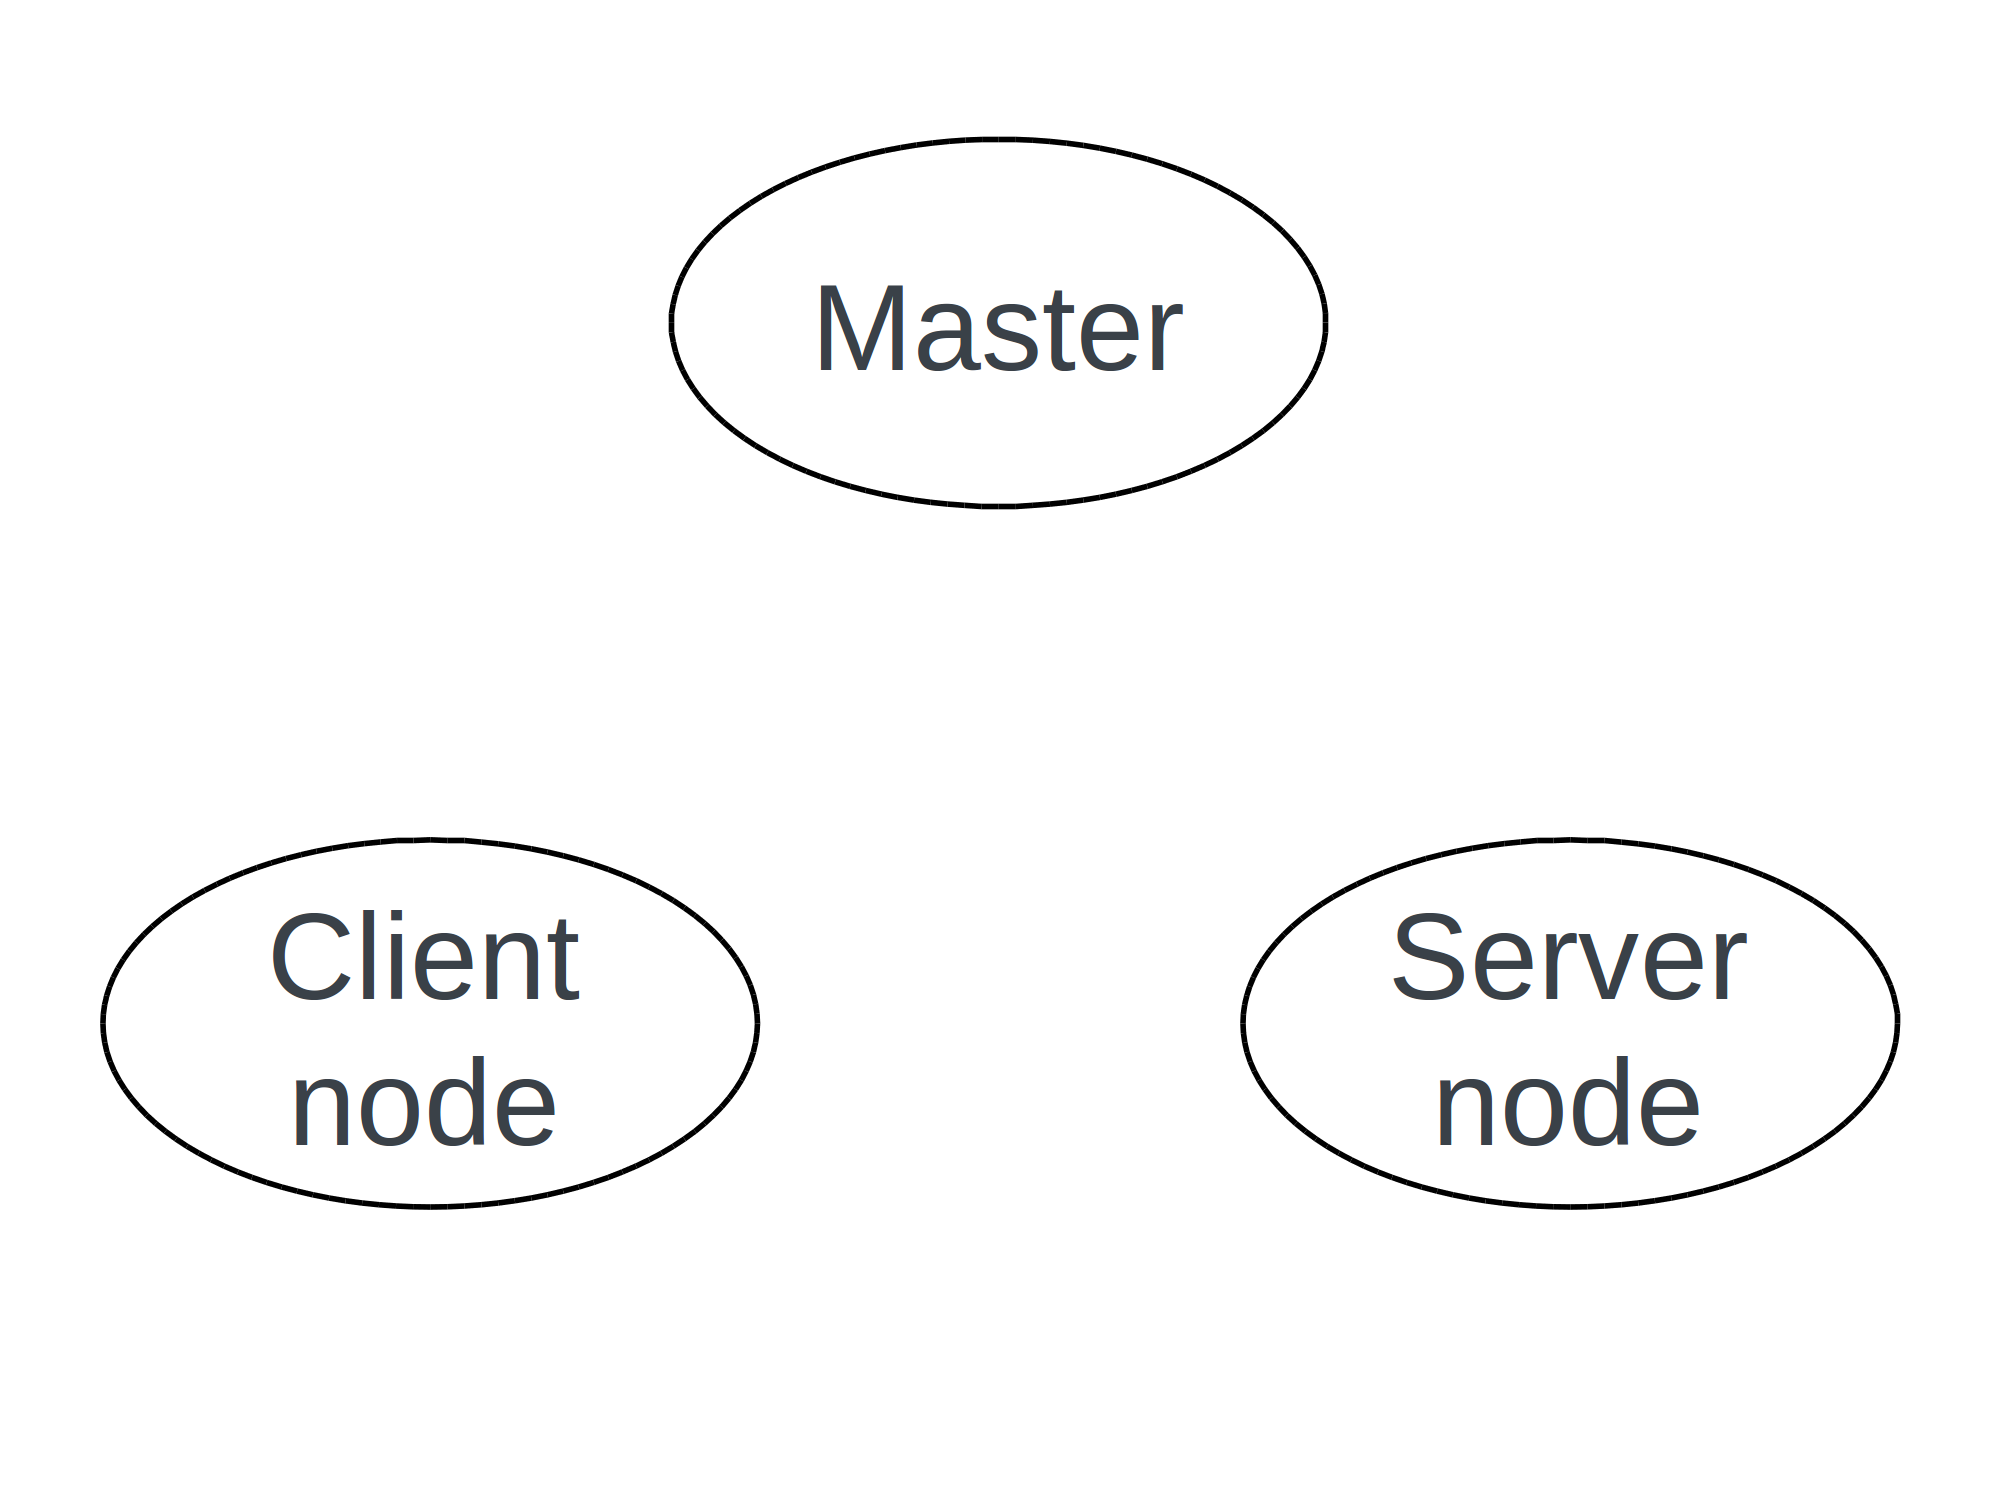
\includegraphics[width =1.0\linewidth]{figures/service1.png}                                                              
  \end{frame}       

\subsection{TurtleSim Services}

\begin{frame}{ROS Services}
    \framesubtitle{TurtleSim Services}
    \begin{itemize}
        \item The {\ttfamily turtlesim} node also acts as a server of multiple ROS services.
        \item To check for ROS services currently being served:
    \begin{terminal}
        \color{green} \ttfamily{rosservice list}
    \end{terminal}
    \end{itemize}
\end{frame}

\setbeamercolor{background canvas}{bg=black}
\begin{frame}[plain]{}  
    \centering
    {\huge \textcolor{white}{Example \\ (TurtleSim services)} }
\end{frame}
\setbeamercolor{background canvas}{bg=white} 

\begin{frame}{ROS Services}
    \framesubtitle{TurtleSim Services}
    \begin{itemize}
        \item To see more information on a service:
       \begin{terminal}
           \color{green} \ttfamily{rosservice info <service name>}
        \end{terminal} 
        \item Example:   
               \begin{terminal}
                   \color{green} \ttfamily{rosservice info /turtle1/set\_pen}
               \end{terminal}      
    \end{itemize}
    \end{frame}

\begin{frame}{ROS Services}
    \framesubtitle{TurtleSim Services}
    \begin{itemize}
        \item To see information on a service type:
        \begin{terminal}
            \color{green} \ttfamily{rossrv show <package/srv>}
        \end{terminal}  
        \item Example:  
        \begin{terminal}
            \color{green} \ttfamily{rossrv show turtlesim/SetPen}
        \end{terminal}  
     \end{itemize}
\end{frame}

\begin{frame}{ROS Services}
    \framesubtitle{TurtleSim Services}
    \begin{itemize}
        \item The output to previous command:
        \begin{terminal}
            \color{green} \ttfamily{
uint8 r\\
uint8 g\\
uint8 b\\
uint8 width\\
uint8 off\\
\textemdash\textemdash\textemdash\\
\\
     }
        \end{terminal}  
    \end{itemize}
\end{frame}

\begin{frame}{ROS Services}
    \framesubtitle{TurtleSim Services}
    \begin{itemize}
        \item To call a service:
        \begin{terminal}
            \color{green} \ttfamily{rosservice call <service name> <request>}
        \end{terminal} 
        
        \item Example:         
    \end{itemize}
            \begin{terminal}
                \color{green} \ttfamily{\tiny{rosservice call /turtle1/set\_pen "{r: 255, g: 255, b: 0, width: 5, 'off': 0}"}}
            \end{terminal} 
            
            \begin{itemize}
                \item Note: use command auto-completion by clicking \keys{Tab} key twice.
            \end{itemize}
\end{frame}

\setbeamercolor{background canvas}{bg=yellow}
\begin{frame}[plain]{}  
    \centering
    {\huge \textcolor{black}{Exercise 1}}
\end{frame}
\setbeamercolor{background canvas}{bg=white}
    
\subsection{Service Description Files}

\begin{frame}{Service Description Files}
\framesubtitle{.srv file format}
\begin{itemize}
    \item A service is defined in a text file with  {\ttfamily \colorbox{yellow}{.srv}} extension.
    \item {\ttfamily \colorbox{yellow}{.srv}} files  must be placed in {\ttfamily \colorbox{gray!30!white}{srv}} folder inside the package.
\end{itemize}
\vspace{5mm}
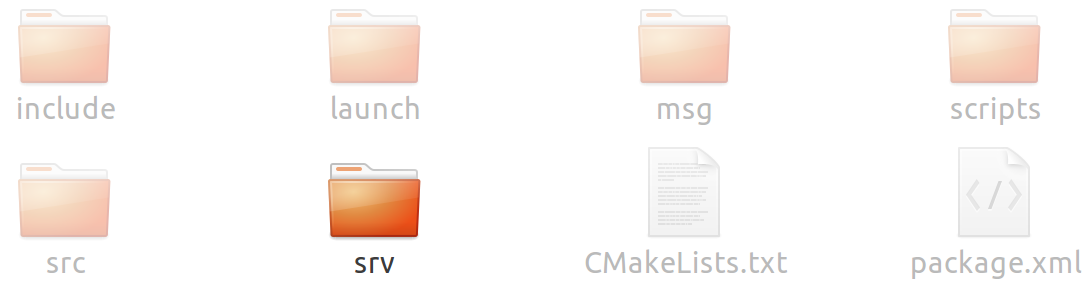
\includegraphics[width=1\linewidth]{figures/package.png}
\end{frame}

\begin{frame}{Service Description Files}
    \framesubtitle{.srv file format}
    \begin{itemize}
        \item To see the services defined in a package:
        \begin{terminal}
            \color{green} \ttfamily{rossrv package <package name>}
        \end{terminal} 
        
        \item Example
        \begin{terminal}
            \color{green} \ttfamily{rossrv package turtlesim}
        \end{terminal} 
    \end{itemize}      
\end{frame}

\begin{frame}{Service Description Files}
    \framesubtitle{.srv file format}
    \begin{itemize}
        \item The file consists of two parts: \textbf{request} message, and \textbf{response} message.
        \item request and response are separated with "\ttfamily{\textemdash\textemdash\textemdash}".
        \begin{focus}
            \ttfamily{
            fieldtype  \hspace{0.5cm} fieldname\\
            fieldtype  \hspace{0.5cm} fieldname\\
            \textemdash \textemdash \textemdash \\
            fieldtype  \hspace{0.5cm} fieldname\\
            fieldtype  \hspace{0.5cm} fieldname}
        \end{focus}
    \end{itemize} 
    \begin{itemize}
        \item Field type can be a ROS built-in type or a defined ROS message. \beamerbutton{\href{http://wiki.ros.org/msg}{Built-in types}} 
    \end{itemize}    
     
\end{frame}

\begin{frame}{Service Description Files}
    \framesubtitle{.srv file format}
    \begin{itemize}
        \item We saw earlier the {\ttfamily{\colorbox{yellow}{turtlesim/SetPen}}} service description:
        \begin{focus}
            \ttfamily
            uint8  \hspace{0.5cm} r\\
            uint8  \hspace{0.5cm} g\\
            uint8  \hspace{0.5cm} b\\
            uint8  \hspace{0.5cm} width\\
            uint8  \hspace{0.5cm} off\\
            \textemdash \textemdash \textemdash \\
            \\
        \end{focus} 
    \end{itemize}      
\end{frame}

\begin{frame}{Service Description Files}
    \framesubtitle{.srv file format}
    \begin{itemize}
        \item Question: if we modify our "useless" node to use services...\\ \vspace{10mm}     how would the service file look like?
    \end{itemize}             
\end{frame}


\begin{frame}{Service Description Files}
    \framesubtitle{.srv file format}
    \begin{itemize}
        \item It could be something like this: \vspace{5mm}
        \begin{focus}
            \ttfamily
            string  \hspace{0.5cm} str\\
            \textemdash \textemdash \textemdash \\
            string  \hspace{0.5cm} str\\
        \end{focus} 
    \end{itemize}      
\end{frame}


\begin{frame}{Service Description Files}
    \framesubtitle{.srv file format}
    \begin{itemize}
        \item When you build your package, Catkin reads {\ttfamily \colorbox{yellow}{.srv}} files and generates Python classes for you.
        \vspace{5mm}
        \item you can use the generated Python classes to define a service server, or service client in your node.
        \vspace{5mm}
        \item We will write a custom service file and do the build process later (but it's exactly similar to ROS messages)...
    \end{itemize}      
\end{frame}


\setbeamercolor{background canvas}{bg=yellow}
\begin{frame}[plain]{}  
    \centering
    {\huge \textcolor{black}{Exercise 2}}
\end{frame}
\setbeamercolor{background canvas}{bg=white}




\subsection{Service Client in Python}

\begin{frame}[fragile]{Service Client in Python}
    \framesubtitle{   ../scripts/01\_simple\_client.py}
    \lstset{language=python,
        basicstyle=\scriptsize,
        keywordstyle=\color{blue}\ttfamily,
        stringstyle=\color{red}\ttfamily,
        commentstyle=\color{green}\ttfamily,
        morecomment=[l][\color{magenta}]{\#},
        showstringspaces=false
    }
    \begin{lstlisting}
    #!/usr/bin/env python
    
    import rospy
    from turtlesim.srv import SetPen
    
    
    if __name__ == '__main__':
    
        rospy.init_node('I_am_client') 
        
        rospy.wait_for_service('/turtle1/set_pen')
        
        pen = rospy.ServiceProxy('/turtle1/set_pen', SetPen)
        
        response = pen(255,0,0,10,0)

    \end{lstlisting}
\end{frame}

\begin{frame}[fragile]{Service Client in Python}
    \framesubtitle{   ../scripts/02\_simple\_client.py}
    \lstset{language=python,
        basicstyle=\scriptsize,
        keywordstyle=\color{blue}\ttfamily,
        stringstyle=\color{red}\ttfamily,
        commentstyle=\color{green}\ttfamily,
        morecomment=[l][\color{magenta}]{\#},
        showstringspaces=false
    }
    \begin{lstlisting}
    #!/usr/bin/env python
    
    import rospy
    from turtlesim.srv import SetPen
    
    if __name__ == '__main__':
    
        rospy.init_node('I_am_client')
        rospy.wait_for_service('/turtle1/set_pen')
        pen = rospy.ServiceProxy('/turtle1/set_pen', SetPen)
        
        try:
            pen(255,0,0,10,0)       
        except rospy.ServiceException, error:
            print "ops! call has failed with this error: ", error 
    
    \end{lstlisting}
\end{frame}

\setbeamercolor{background canvas}{bg=yellow}
\begin{frame}[plain]{}  
    \centering
    {\huge \textcolor{black}{Exercise 3}}
\end{frame}
\setbeamercolor{background canvas}{bg=white}
    
    
    
\begin{frame}[fragile]{Service Client in Python}
    \framesubtitle{ServiceProxy class}
    \begin{focus}
        
        \ttfamily rospy.ServiceProxy(\\
        {\color{red}name},\\
        {\color{red}service\_class},\\
        {\color{blue}persistent=False},\\
        {\color{blue}headers=None}\\
        )
    \end{focus}
\begin{itemize}
        \item Let's check this class definition in rospy!
        \beamerbutton{
            \href{http://docs.ros.org/kinetic/api/rospy/html/rospy.impl.tcpros_service.ServiceProxy-class.html}{ServiceProxy class}
            }
        \item there is a {\ttfamily \colorbox{yellow}{wait\_for\_service}} method in the class, let's try it!
    \end{itemize}        
\end{frame}
    
\begin{frame}[fragile]{Service Client in Python}
    \framesubtitle{   ../scripts/03\_simple\_client.py}
    \lstset{language=python,
        basicstyle=\scriptsize,
        keywordstyle=\color{blue}\ttfamily,
        stringstyle=\color{red}\ttfamily,
        commentstyle=\color{green}\ttfamily,
        morecomment=[l][\color{magenta}]{\#},
        showstringspaces=false
    }
    \begin{lstlisting}
    #!/usr/bin/env python
    
    import rospy
    from turtlesim.srv import SetPen
    from time import sleep
    
    if __name__ == '__main__':
    
        rospy.init_node('I_am_client') 
        pen = rospy.ServiceProxy('/turtle1/set_pen', SetPen)
        
        pen.wait_for_service()
        
        try:
            pen(255,0,0,10,0)      
        except rospy.ServiceException, error:
            print "ops! call has failed with this error: ", error 
    
    \end{lstlisting}
\end{frame}

    
\subsection{Service Server in Python}

\begin{frame}{Service Server in Python}
    \begin{itemize}
        \item Let's write a service server now!
        \vspace{5mm}
        \item The service file must be defined first, we can use:
        \vspace{5mm}
        \begin{itemize}
            \item \textbf{existing} service files defined in other packages.
        \vspace{2mm}            
            \item write our own \textbf{custom} service file.
        \end{itemize}
        \vspace{2mm}            
        \item The process is the same, but writing/using a custom {\ttfamily \colorbox{yellow}{.srv}} file will be covered next section.\\ \scriptsize{(we already saw how the file looks like, but we need to see how to build the services with Catkin)}
    \end{itemize}      
\end{frame}

\begin{frame}[fragile, plain]{Service Server in Python}
    \framesubtitle{   ../scripts/04\_simple\_server.py}
    \lstset{language=python,
        basicstyle=\ttfamily\scriptsize,
        keywordstyle=\color{blue}\ttfamily,
        stringstyle=\color{red}\ttfamily,
        commentstyle=\color{green}\ttfamily,
        morecomment=[l][\color{magenta}]{\#},
        showstringspaces=false
    }
    \begin{lstlisting}
    #!/usr/bin/env python 
    import rospy
    from std_srvs.srv import SetBool, SetBoolResponse
    
    def destroy(req):
        print "Roger that!.."
        response = SetBoolResponse()
        response.success = True
        if req.data:
            response.message = "You are victorious!"
        else:
            response.message = "enemy spared!"
        return response
    
    if __name__ == '__main__':
        rospy.init_node('red_alert_server')
        print("Ready for melt-down!")
        serv = rospy.Service('destroy_enemy', SetBool, destroy)
        serv.spin()
    \end{lstlisting}
\end{frame}

\begin{frame}[fragile]{Service Server in Python}
    \framesubtitle{Service class}
    \begin{focus}
        
        \ttfamily rospy.Service(\\
        {\color{red}name},\\
        {\color{red}service\_class},\\
        {\color{red} handler},\\
        {\color{blue}buff\_size=65536},\\
        {\color{blue} error\_handler=None}\\
        )
    \end{focus}
    \begin{itemize}
        \item Let's check this class definition in rospy!
        \beamerbutton{
            \href{http://docs.ros.org/kinetic/api/rospy/html/rospy.impl.tcpros_service.Service-class.html}{Service class}
        }
    \end{itemize}        
\end{frame}

\setbeamercolor{background canvas}{bg=yellow}
\begin{frame}[plain]{}  
    \centering
    {\huge \textcolor{black}{Exercise 4}}
\end{frame}
\setbeamercolor{background canvas}{bg=white}


\subsection{Using a Custom Service}

\begin{frame}{Using a Custom Service}
    \begin{itemize}
        \item We already have seen how to write an {\ttfamily \colorbox{yellow}{.srv}} file.

        \vspace{5mm}

        \item Let's write an {\ttfamily \colorbox{yellow}{.srv}} file for our "useless" node, and tell Catkin to build it.
    \end{itemize}
\end{frame}

\begin{frame}{Using a Custom Service}
    \framesubtitle{our custom .srv file}
    \begin{focus}
        \ttfamily
        string  \hspace{0.5cm} str\\
        \textemdash \textemdash \textemdash \\
        string  \hspace{0.5cm} str\\
    \end{focus} 
    \vspace{2mm}
    \begin{itemize}
        \item To tell Catkin to build our service, we (again) need to modify {\ttfamily \colorbox{yellow}{CMakeList.txt}} and {\ttfamily \colorbox{yellow}{package.xml}} files of our package.
        \vspace{2mm}
        \item It's similar to what we did for custom messages.
    \end{itemize}      
\end{frame}

\begin{frame}{Using a Custom Service}
    \framesubtitle{package.xml changes}

    The changes that we should make to {\ttfamily \colorbox{yellow}{package.xml}}:
    \begin{enumerate}
        \item Add dependencies on message generation:
    \end{enumerate}  
    \begin{focus}
        \ttfamily \scriptsize
        {\color{blue}<build\_depend>} message\_generation {\color{blue}</build\_depend>}\\
        
        {\color{blue}<build\_depend>} message\_runtime {\color{blue}</build\_depend>}\\
    \end{focus}         
\end{frame}

\begin{frame}{Using a Custom Service}
    \framesubtitle{CMakeList.txt changes}
    
    The changes that we should make to {\ttfamily \colorbox{yellow}{CMakeList.txt}}:
    \vspace{5mm}
    \scriptsize
    \begin{enumerate}
        \item add {\ttfamily \colorbox{gray!30!white}{message\_generation}} to {\ttfamily \colorbox{gray!30!white}{find\_package()}} under {\ttfamily \colorbox{gray!30!white}{COMPONENTS}}.
        \vspace{2mm}
        
        \item  add {\ttfamily \colorbox{gray!30!white}{message\_runtime}} to {\ttfamily \colorbox{gray!30!white}{catkin\_package()}} under {\ttfamily \colorbox{gray!30!white}{CATKIN\_DEPENDS}}.
        \vspace{2mm}
        
        \item add service file(s): (our {\ttfamily \colorbox{yellow}{.srv}} file should be in the {\ttfamily \colorbox{gray!30!white}{srv}} folder in package directory, else it will cause an error):
        \vspace{2mm}
        \begin{focus}
            \ttfamily \scriptsize
            add\_service\_files(\\
            FILES\\
            ourFile.srv\\
            )
          \end{focus}  
   \end{enumerate}
        
\end{frame}

\begin{frame}{Using a Custom Service}
    \framesubtitle{CMakeList.txt changes}
    
    \scriptsize
    \begin{enumerate}
        \setcounter{enumi}{3}
        \item generate messages, and add all dependencies you used in {\ttfamily \colorbox{yellow}{srv}} file:
        \begin{focus}
            \ttfamily \scriptsize
            generate\_messages(\\
            DEPENDENCIES\\
            std\_msgs\\
            )
        \end{focus}  
        
    \end{enumerate}
    
    \begin{itemize}
        \item Note: {\ttfamily \colorbox{gray!30!white}{add\_service\_files()}} and {\ttfamily \colorbox{gray!30!white}{generate\_messages()}} need to be called before {\ttfamily \colorbox{gray!30!white}{catkin\_packge()}}, else will error.
    \end{itemize}
    
\end{frame}

\setbeamercolor{background canvas}{bg=yellow}
\begin{frame}[plain]{}  
    \centering
    {\huge \textcolor{black}{Exercise 5}}
\end{frame}
\setbeamercolor{background canvas}{bg=white}


\setbeamercolor{background canvas}{bg=yellow}
\begin{frame}[plain]{}  
    \centering
    {\huge \textcolor{black}{Exercise 6}}
\end{frame}
\setbeamercolor{background canvas}{bg=white}

\section{References}
\begin{frame}{References}

    \begin{enumerate}
        \item rospy full documentation.

        \url{http://docs.ros.org/kinetic/api/rospy/html/}
        
        \item \href{http://wiki.ros.org/ROS/Tutorials/WritingServiceClient(python)}{ROS Wiki {\scriptsize/ WritingServiceClient(python)}}. 
        
        \item \href{https://github.com/mas-group/minimal_ros_packages/tree/master/srv_minimal}{MAS {\ttfamily \colorbox{gray!30!white}{minimal\_ros\_packages}} GitHub repository}. {\tiny(build instructions, exact copy) }       
        
        \item \href{http://docs.ros.org/kinetic/api/catkin/html/howto/format2/building_msgs.html}{Catkin Documentation {\scriptsize/ building\_msgs}}
    \end{enumerate}
\end{frame}



\setbeamercolor{background canvas}{bg=black}
\begin{frame}[plain]{}  
    \centering
    {\huge \textcolor{white}{Thank you}}
    
    \vspace{0.5cm}
    
    {\huge \textcolor{white}{Any questions?}}
\end{frame}
\setbeamercolor{background canvas}{bg=white}


\end{document}
